\documentclass{article}
\usepackage{amsmath,tikz,pgfplots}
\pgfplotsset{compat=1.16}
\usepgfplotslibrary{fillbetween}
\title{MATH 200 Assignment Two}
\author{%
	Oliver Tonnesen\\
	V00885732\\
	A02 \-- T03}
\date{October 16, 2018}
\begin{document}
\maketitle
\section{} % Question 1
	Recall the curvature formula:
	\[\kappa=\frac{|f''(x)|}{{\big(1+|f'(x)|^2\big)}^{\frac{3}{2}}}\]
	We will use this formula with $f(x)=e^x$:
	\begin{align*}
		\kappa&=\frac{|f''(x)|}{{\big(1+|f'(x)|^2\big)}^{\frac{3}{2}}}\\
		&=\frac{|e^x|}{{\big(1+|e^x|^2\big)}^\frac{3}{2}}\\
		&=\frac{e^x}{{\big(1+e^{2x}\big)}^\frac{3}{2}}&\text{($e^x>0$ for all $x$)}
	\end{align*}
	So the curvature of $f(x)$ is $\frac{e^x}{{\big(1+e^{2x}\big)}^\frac{3}{2}}$, and we can now use basic calculus to find
	its maximum:
	\begin{align*}
		\frac{d}{dx}\Bigg(\frac{e^x}{{\big(1+e^{2x}\big)}^\frac{3}{2}}\Bigg)&=e^x\cdot{\big(1+e^2x\big)}^{-\frac{3}{2}}-3e^{3x}\cdot{\big(1+e^{2x}\big)}^{-\frac{5}{2}}\\
		&=\frac{e^x}{{\big(1+e^{2x}\big)}^\frac{5}{2}}\Bigg(\big(1+e^{2x}\big)-3e^{2x}\Bigg)\\
		&=\frac{e^x}{{\big(1+e^{2x}\big)}^\frac{5}{2}}\Big(1-2e^{2x}\Big)\\
		&=\frac{e^x-2e^{3x}}{{\big(1+e^{2x}\big)}^\frac{5}{2}}
	\end{align*}
	We find the critical points:
	\begin{align*}
		\frac{e^x-2e^{3x}}{{\big(1+e^{2x}\big)}^\frac{5}{2}}&=0\\
		e^x-2e^{3x}&=0\\
		e^x&=2e^{3x}\\
		1&=2e^{2x}&\text{($e^x\neq{0}$ for all $x$)}\\
		e^{2x}&=\frac{1}{2}\\
		e^x&=\frac{1}{\sqrt{2}}\\
		x&=\ln{\bigg(\frac{1}{\sqrt{2}}\bigg)}
	\end{align*}
	So the point of maximum curvature for the curve $y=e^x$ is at $x=\frac{1}{\sqrt2}$.
	We will now find the curvature's behavior as $x\to\infty$:
	\[\lim_{x\to\infty}\frac{e^x}{{\big(1+e^{2x}\big)}^{\frac{3}{2}}}\]
	Note first that both the numerator and the denominator are always greater than zero, and so
	the fraction can never be less than zero.
	\begin{align*}
		\lim_{x\to\infty}\frac{e^x}{{\big(1+e^{2x}\big)}^{\frac{3}{2}}}&=\lim_{x\to\infty}\frac{e^x}{{\bigg[{\big(1+e^{2x}\big)}^3\bigg]}^\frac{1}{2}}\\
		&=\lim_{x\to\infty}\frac{e^x}{{\big(1+3e^{2x}+3e^{4x}+e^{6x}\big)}^{\frac{1}{2}}}\\
		&\le\lim_{x\to\infty}\frac{e^x}{{\big(e^{6x}\big)}^\frac{1}{2}}\\
		&=\lim_{x\to\infty}\frac{e^x}{e^{3x}}\\
		&=\lim_{x\to\infty}\frac{1}{e^{2x}}\\
		&=0
	\end{align*}
	So the curvature is less than or equal to a similar function that goes to zero.
	Recall that our curvature is always greater than zero, so the curvature goes to
	zero as x goes to infinity.
\section{} % Question 2
	\[f(x,y)=\frac{\sqrt{y-x^2}}{1-x^2}\]
	So our constraints on $x$ and $y$ are:
	\begin{align*}
		y-x^2&\ge0\\
		y&\ge{x^2}
	\end{align*}
	since the square root of a negative number is undefined, and
	\begin{align*}
		1-x^2&\neq0\\
		x^2&\neq1\\
		x&\neq\pm1
	\end{align*}
	since division by zero is undefined.
	So our domain is the region above and including the parabola $y=x^2$ with removable discontinuities at
	$x=1$ and $x=-1$:\\\\
	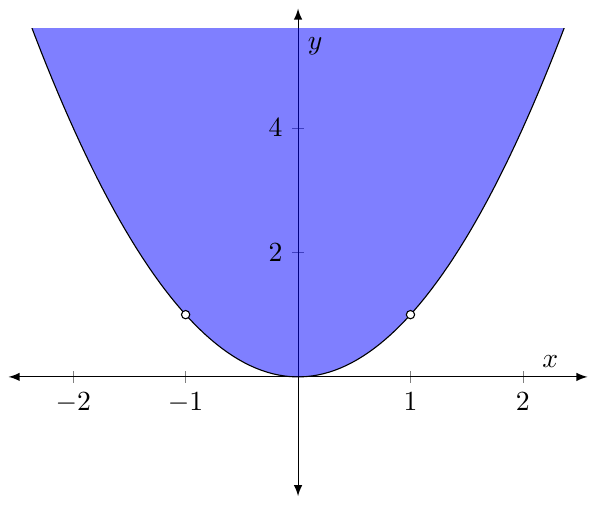
\begin{tikzpicture}
	\begin{axis}[
			xmin=-2,xmax=2,
			ymin=-1,ymax=5,
			xlabel={$x$},
			ylabel={$y$},
			axis lines=middle,
			enlargelimits,
			axis line style={shorten >=-0.25cm,shorten <=-0.25cm,latex-latex},
			extra x tick style={grid=none}
			]
		\addplot[name path=f,domain=-5:5,mark=none,samples=200]{x^2};
		\addplot[name path=bound,domain=-3:3,mark=none]{6};
		\addplot[
			thick,
			color=blue,
			fill=blue,
			fill opacity=0.5
			] fill between [
				of=f and bound,
				];

		\draw[fill=white] (axis cs:-1,1) circle [radius=1.5pt];
		\draw[fill=white] (axis cs:1,1) circle [radius=1.5pt];
	\end{axis}
	\end{tikzpicture}
\section{} % Question 3
	We'll sketch the isothermals at $T(x,y)=1,2,3,4$.
	$T(x,y)=1$:
	\begin{align*}
		1&=\frac{100}{1+x^2+2y^2}\\
		1+x^2+2y^2&=100\\
		x^2+2y^2&-99=0\\
	\end{align*}
	The same process can be repeated for $T(x,y)=2,3,4$:\\\\
	$T(x,y)=2$:
	\[2x^2+4y^2-98=0\]
	$T(x,y)=3$:
	\[3x^2+6y^2-97=0\]
	$T(x,y)=4$:
	\[4x^2+8y^2-96=0\]
	\\\\
	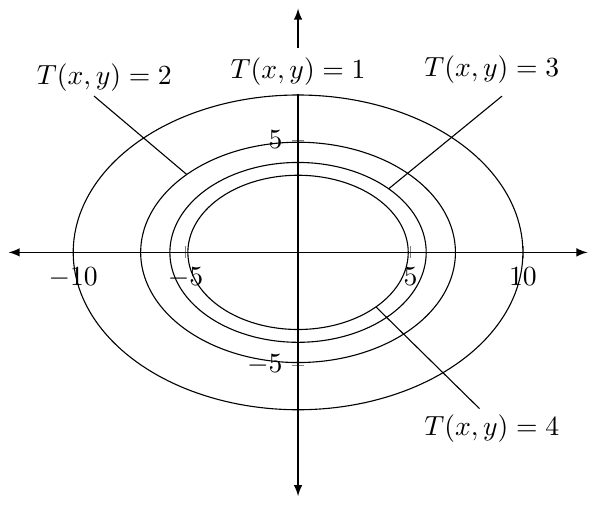
\begin{tikzpicture}
	\begin{axis}[
		xmin=-10,xmax=10,
		ymin=-7,ymax=7,
		axis equal,
		axis x line=middle,
		axis y line=middle,
		enlargelimits,
		axis line style={shorten >=-0.25cm,shorten <=-0.25cm,latex-latex},
		]
		\addplot[domain=0:360,samples=200]({10*sin(x)},{7*cos(x)}) node[fill=white,above]{$T(x,y)=1$};
		\addplot[domain=0:360,samples=200]({7*sin(x)},{4.9*cos(x)}) node[fill=white,above,xshift=-70pt,yshift=15pt]{$T(x,y)=2$};
		\addplot[domain=0:360,samples=200]({5.7*sin(x)},{4*cos(x)}) node[fill=white,above,xshift=70pt,yshift=25pt]{$T(x,y)=3$};
		\addplot[domain=0:360,samples=200]({4.9*sin(x)},{3.43*cos(x)}) node[fill=white,above,xshift=70pt,yshift=-100pt]{$T(x,y)=4$};
		\draw (axis cs:{7*sin(315)},{4.9*cos(315)}) -- (axis cs:{10*sin(315)-2},{7*cos(315)+2});
		\draw (axis cs:{5.7*sin(45)},{4*cos(45)}) -- (axis cs:{10*sin(45)+2},{7*cos(45)+2});
		\draw (axis cs:{4.9*sin(135)},{3.43*cos(135)}) -- (axis cs:{10*sin(135)+1},{7*cos(135)-2});

	\end{axis}
	\end{tikzpicture}
\section{} % Question 4
	We consider two lines: $\{(x,y)|x=z^2,y=z^2\}$ and $\{(x,y)|x=z^2,y=0\}$.\\\\
	$\{(x,y)|x=z^2,y=z^2\}$:
	\begin{align*}
		&\lim_{z\to0}\frac{(z^2)(z^2)+(z^2)z^2+(z^2)z^2}{{(z^2)}^2+{(z^2)}^2+z^4}\\
		&=\lim_{z\to0}\frac{3z^4}{3z^4}\\
		&=\lim_{z\to0}\frac{1}{1}\\
		&=1\\
	\end{align*}
	$\{(x,y)|x=z^2,y=0\}$:
	\begin{align*}
		&\lim_{z\to0}\frac{(z^2)(0)+(0)z^2+(z^2)z^2}{{(z^2)}^2+{(0)}^2+z^4}\\
		&=\lim_{z\to0}\frac{0+0+z^4}{z^4+0+z^4}\\
		&=\lim_{z\to0}\frac{z^4}{2z^4}\\
		&=\lim_{z\to0}\frac{1}{2}\\
		&=\frac{1}{2}\\
	\end{align*}
	$1\neq\frac{1}{2}$, so the limit does not exist.
\section{} % Question 5
	First we define the function $z(x,y)=x^2+y^2$. (Note that $\lim_{(x,y)\to(0,0)}z(x,y)=0$) Then
	\begin{align*}
		\lim_{(x,y)\to(0,0)}\frac{e^{-x^2-y^2}-1}{x^2+y^2}&=\lim_{z\to0}\frac{e^{-z}-1}{z}\\
		&=\lim_{z\to0}\frac{-e^{-z}}{1}&\text{(L'H\^{o}pital's Rule)}\\
		&=-e^{-0}\\
		&=-e^0\\
		&=-1
	\end{align*}
\section{} % Question 6
	\begin{align*}
		\frac{\partial{w}}{\partial{x}}&=\frac{1}{x+2y+3z}\\\\
		\frac{\partial{w}}{\partial{y}}&=\frac{2}{x+2y+3z}\\\\
		\frac{\partial{w}}{\partial{z}}&=\frac{3}{x+2y+3z}
	\end{align*}
\section{} % Question 7
	Recall Clairaut's Theorem:\\
	Suppose $f$ is defined on a disk $D$ that contains $(a,b)$. If $f_{xy}$ and $f_{yx}$
	are both continuous on $D$, then $f_{xy}(a,b)=f_{yx}(a,b)$.
	\begin{align*}
		\frac{\partial{f}}{\partial{x}}&=ye^{xy}\sin{y}\\
		\frac{\partial^2{f}}{\partial{x}\partial{y}}&=e^{xy}\sin{y}+yxe^{xy}\sin{y}+ye^{xy}\cos{y}\\
		\frac{\partial{f}}{\partial{y}}&=xe^{xy}\sin{y}+e^{xy}\cos{y}\\
		\frac{\partial^2{f}}{\partial{y}\partial{x}}&=xye^{xy}\sin{y}+e^{xy}\sin{y}+ye^{xy}\cos{y}\\
	\end{align*}
	We find that $\frac{\partial^2{f}}{\partial{x}\partial{y}}=\frac{\partial^2{f}}{\partial{y}\partial{x}}$,
	and so Clairaut's Theorem holds.
\section{} % Question 8
	\begin{align*}
		\frac{\partial{z}}{\partial{u}}&={(v-w)}^\frac{1}{2}\\
		\frac{\partial^2{z}}{\partial{u}\partial{v}}&=\frac{1}{2}{(v-w)}^{-\frac{1}{2}}\\\\
		\frac{\partial^3{z}}{\partial{u}\partial{v}\partial{w}}&=\frac{1}{4}{(v-w)}^{-\frac{3}{2}}\\
	\end{align*}
\section{} % Question 9
	Recall the Law of Cosines:\\
	\[a^2=b^2+c^2+2bc\cos{\big(A\big)}\]
	\[A=\arccos{\Big(\frac{a^2-b^2-c^2}{2bc}\Big)}\]
	\begin{align*}
		\frac{\partial{A}}{\partial{a}}&=-\frac{\frac{2a}{2bc}}{\sqrt{1-{\big(\frac{a^2-b^2-c^2}{2bc}\big)}^2}}\\
		&=-\frac{a}{bc\sqrt{1-{\big(\frac{a^2-b^2-c^2}{2bc}\big)}^2}}\\\\
		\frac{\partial{A}}{\partial{b}}&=-\frac{\frac{-a^2-b^2+c^2}{2cb^2}}{\sqrt{1-{\big(\frac{a^2-b^2-c^2}{bc}\big)}^2}}\\
		&=\frac{a^2+b^2-c^2}{2cb^2\sqrt{1-{\big(\frac{a^2-b^2-c^2}{bc}\big)}^2}}\\\\
		\frac{\partial{A}}{\partial{c}}&=-\frac{\frac{-a^2+b^2-c^2}{2bc^2}}{\sqrt{1-{\big(\frac{a^2-b^2-c^2}{bc}\big)}^2}}\\
		&=\frac{a^2-b^2+c^2}{2bc^2\sqrt{1-{\big(\frac{a^2-b^2-c^2}{bc}\big)}^2}}\\
	\end{align*}
\end{document}
